\section{Methods}
\label{sec:Methods}

\subsection{Model description}
\label{subsec:Model}

We focused our attention on food webs with two trophic levels, competing prey and predators. The predators (consumers) have a differentiated preference of different prey species.

% Description of the dynamics
The dynamics were modelled using the Rosenzweig-MacArthur predator-prey model \citep{Rosenzweig1963}, generalized to a higher number of species \citep{Scheffer2004}. Our model contains $n_P$ prey species and $n_C$ predator species. The prey’s populations are under the influence of both intra and interspecific competition, whose intensities are defined by the competition matrix $A$. The relative preference that predators have for each prey is defined by the predation matrix $S$. Prey immigration from neighboring areas has been added to the classical model in order to avoid unrealistic dynamics, such as heteroclinic orbits giving rise to long-stretched cycles with near extinctions \citep{Scheffer2004}. In mathematical notation, the system reads:
%
\begin{eqnarray}
\label{eq:SystemUnderStudy}
	\begin{cases}
	\frac{dP_i}{dt} =  r_i(P) P_i  - \sum_{j = 1}^{n_C} g_j(P) P_i S_{ji} C_j + f & : i = 1..n_P
	\\
	\frac{dC_j}{dt} = - l C_j +  e \sum_{i = 1}^{n_P} g_j(P) P_i S_{ji} C_j  & : j = 1..n_C
	\end{cases}
\end{eqnarray}
%
where $P_i(t)$ represents the biomass of prey species $i$ at time $t$ and $C_j(t)$ the biomass of predator species $j$ at time $t$. The symbol $P$ is used as a shorthand for the vector $(P_1(t), P_2(t), ..., P_{n_P}(t))$. The auxiliary functions $r_i(P)$ and $g_j(P)$ (see equations \eqref{eq:LogisticGenerator} and \eqref{eq:HollingGenerator}) have been respectively chosen to generalize the logistic growth and the Holling type II saturation functional response \citep{Edelstein-Keshet} to a multispecies system when inserted into equation \eqref{eq:SystemUnderStudy}.
%
\begin{equation}
\label{eq:LogisticGenerator}
	r_i(P) = r \left( 1 - \frac{1}{K} \sum_{k=1}^{n_P} A_{ik} P_k \right)
\end{equation}
%
\begin{equation}
\label{eq:HollingGenerator}
	g_j(P) = \frac{g}{\sum_{i=1}^{n_P} S_{ji} P_i + H}
\end{equation}
%
For details about the parameters used, please refer to subsection \ref{subsec:Parameterization}.

\subsection{Parameterization}
\label{subsec:Parameterization}
We parameterized our model as a freshwater plankton system based on Dakos' model \citep{Dakos2009b}. Unlike Dakos, who uses seasonally changing parameters, our parameters were assumed to be independent of time (see table \ref{tab:Parameters}).

\begin{table}[H]
	\begin{center}
		\resizebox{\columnwidth}{!}{
		\begin{tabular}{cccc}
			\hline
			\textbf{Symbol} & \textbf{Interpretation} & \textbf{Value} & \textbf{Units} \\
			\hline
			$r$ & Maximum growth rate & $0.50$ & $d^{-1}$ \\
		    \hline
			$K$ & Carrying capacity & $10.00$ & $ mg \ l^{-1} $ \\
			\hline
			$g$ & Predation rate & $0.40$ & $d^{-1}$\\
			\hline
			$f$ & Immigration rate & $10^{-5}$ & $mg \ l^{-1} \ d^{-1}$\\
			\hline
			$e$ & Assimilation efficiency & $0.60$ & $1$\\
			\hline
			$H$ & Saturation constant & $2.00$ & $ mg \ l^{-1} $\\
		    \hline
			$l$ & Predator's loss rate & $0.15$ & $d^{-1}$\\
			\hline
		    $S$ & $ n_C \times n_P $ predator preference matrix & See section \ref{subsubsec:CompetitionParameter} & $1$\\
		    \hline
   		    $A$ & $ n_P \times n_P $ competition matrix & See section \ref{subsubsec:CompetitionParameter} & $1$\\
		    \hline
		\end{tabular}}
	\end{center}
	\caption{Values and meanings of the parameters used in our numerical experiment. The elements of the predation ($S$) and competition ($A$) matrices are drawn from probability distributions described in subsection \ref{subsubsec:CompetitionParameter}.}
	\label{tab:Parameters}
\end{table}

\subsubsection{Competition and predation matrices}
\label{subsubsec:CompetitionParameter}

Our main purpose is to analyze the effect of different competition strengths on the long term dynamics exhibited. For this, we introduce the competition parameter $\epsilon$ to build a competition matrix $A$, whose non-diagonal terms are drawn from a uniform distribution centered at $1+\epsilon$ and with a given width (here we chose $ w = \windowWidth$). The diagonal terms are by definition 1. Defined this way, the parameter $\epsilon$ allows us to move continuously from strong intraspecific ($ \epsilon < 0$) to strong interspecific competition ($ \epsilon > 0$), meeting near-neutral competition at $\epsilon = 0$. For the rest of this paper, we will call ecosystems with $ \epsilon = 0$, \textit{neutral-on-average} (see figure \ref{fig:CompetitionParameter}).

\begin{figure}[H]
	\begin{center}
		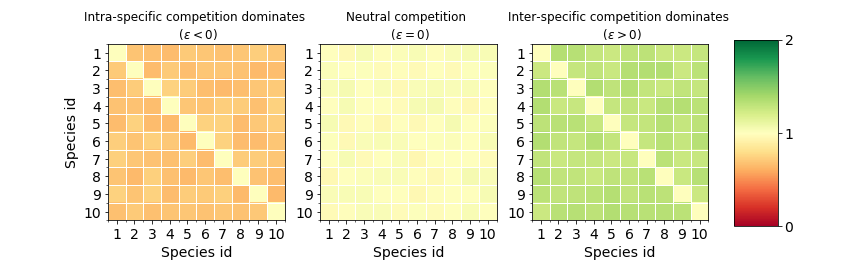
\includegraphics[width=1\columnwidth]{epsilon_all.png}
	\end{center}
	\caption{The competition matrix on the left is a clear case of dominant intraspecific competition. The central one represents a case of neutral-on-average competition. The matrix in the right panel shows a case of dominant interspecific competition. The difference between them is the relative size of the non-diagonal elements respective of the diagonal ones. This property of the competition matrices is controlled by the competition parameter $\epsilon$.}
	\label{fig:CompetitionParameter}
\end{figure}

Regarding the predation matrix $S$ , we follow \citet{Dakos2009b} and draw each of its coefficients from a uniform probability distribution bounded between $0$ and $1$.

\subsection{Numerical experiments}
\label{subsec:NumericalExperiment}

Depending on the parameters and initial conditions, our model (equation \eqref{eq:SystemUnderStudy}) can have three kinds of dynamics, each of them roughly corresponding to a different kind of attractor (see figure \ref{fig:TimeSeries}). In a stable point attractor, species composition is constant. The limit cycle (and limit tori) attractors corresponds to periodically (or quasiperiodically) changing species composition. The last category are chaotic attractors, where the species composition changes irregularly within bounds and there is sensitivity to initial conditions. 

\begin{figure}
	\begin{center}
		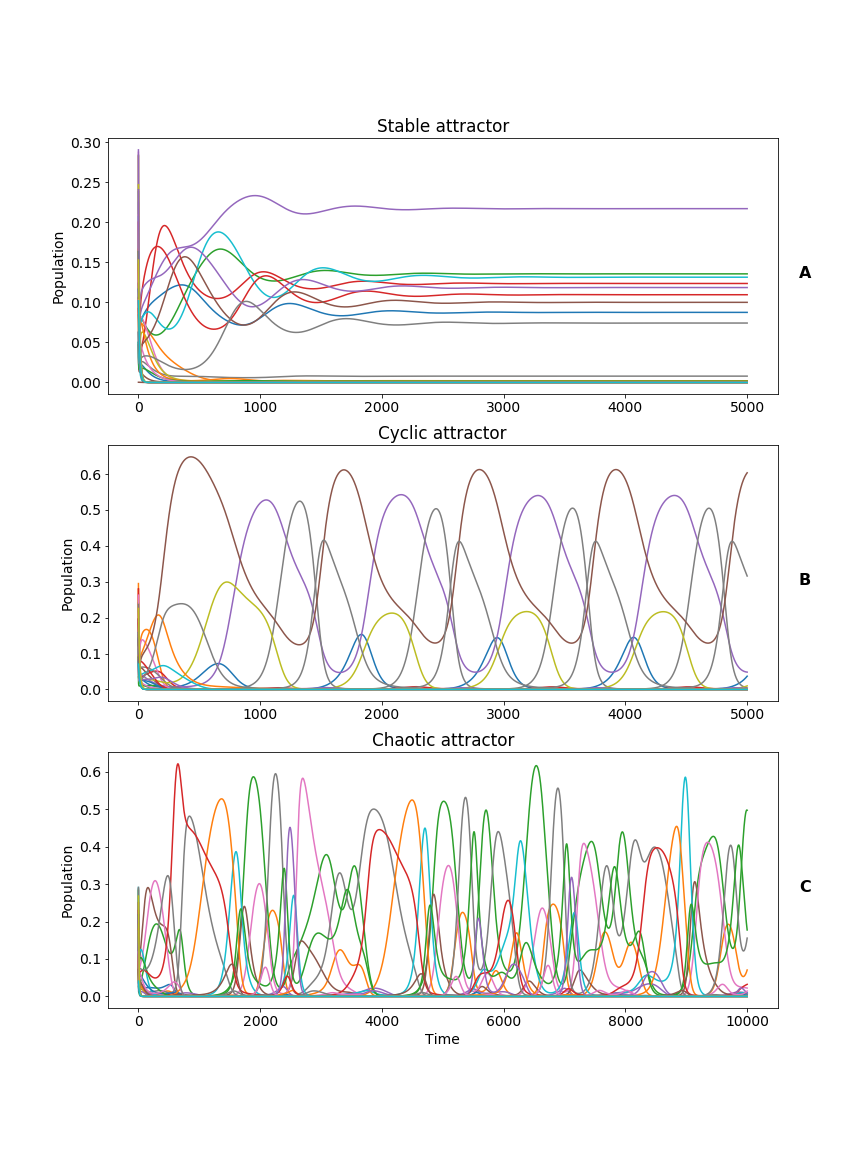
\includegraphics[width=1\columnwidth]{ts.png}
	\end{center}
	\caption{Our family of models generates time series of the population of each species. The time series can be classified in $3$ qualitative types depending on their asymptotic behaviour: \textit{stable}, \textit{cyclic} and \textit{chaotic}. In \textbf{panel A}, the system reaches a stable attractor after a transient time. In \textbf{panel B}, a periodic attractor, with an approximate period of 1000 days, is reached after the transient time. The system in \textbf{panel C} never reaches a stable nor a cyclic attractor, but a chaotic one.}
	\label{fig:TimeSeries}
\end{figure}

% Time series generation
Our target is to estimate the probability of reaching each type of attractor under different assumptions about competition. For this, we analyzed $\numEpsilons$ values of the competition parameter $\epsilon$ (defined in section \ref{subsubsec:CompetitionParameter}), ranging from $\epsilon = -0.8$ to $\epsilon = 0.8$. The lower value was chosen to assure that the non-diagonal competition matrix elements were positive to exclude facilitation. The upper value was arbitrarily chosen to be symmetric with the lower one. For each value of the competition parameter, $\numReps$ different predation and competition matrices were drawn from the probability distributions described in section \ref{subsubsec:CompetitionParameter}. We used a Runge-Kutta solver (ode45) to simulate the model with each parameter set. A stabilizing run of $ \stabilTime $ days was executed to discard transient dynamics. Simulating for $ \simTime $ more days, we obtained a time series close to the attractor.

% Analysis
We determined the fraction of the $\numReps$ time series that were stable, cyclic or chaotic.  For our multi-species models, we found that the Gottwald - Melbourne test \citep{Gottwald2009} was the most reliable test for this classification.  Additionally, two different measures of biodiversity were applied to each simulated ecosystem: the average number of non-extinct prey species and the average biomass grouped by trophic level. We considered a species to be extinct when their population density remained below a threshold of $\bioThreshold$ $mg$ $l^{-1}$ after the stabilization run. We determined the relationship between the competition strength, the probability of each dynamical regime and the biodiversity.

The numerical experiment was repeated for food webs of different sizes, ranging from a total of $5$ to $50$ species. In our simulations, we kept a ratio of 2:3 for the number of species at the consumer and the prey level.

In the spirit of reproducible research, we made available the code used to obtain our conclusions and generate our figures \citep{Rodriguez-Sanchez-code-neuchaos}.